\subsection{Magic 123}\label{Magic123}

``\textbf{One} Image \textbf{to} High-Quality \textbf{3D} Object generation using both 2D and 3D diffusion priors''~\citep{qian2023magic123}~-~Magic123~-~generates 3D meshes using a coarse-to-fine manner as already seen in other methods. The approach is distinctively characterized by its ability to balance between imaginative exploration  using 2D priors and precise exploitation of the generated geometry with 3D priors \citep{qian2023magic123}.

At its core, Magic123 begins with the segmentation of the object from the background using the Dense Prediction Transformer model \citep{ranftl2021vision}. This step extracts the foreground object with its mask, which is then processed further with the MiDaS \citep{ranftl2020robust} model to generate a depth map, preventing the flattening of geometry and capturing the object's actual geometric details \citep{qian2023magic123}.

\begin{figure}[ht]
  \centering
    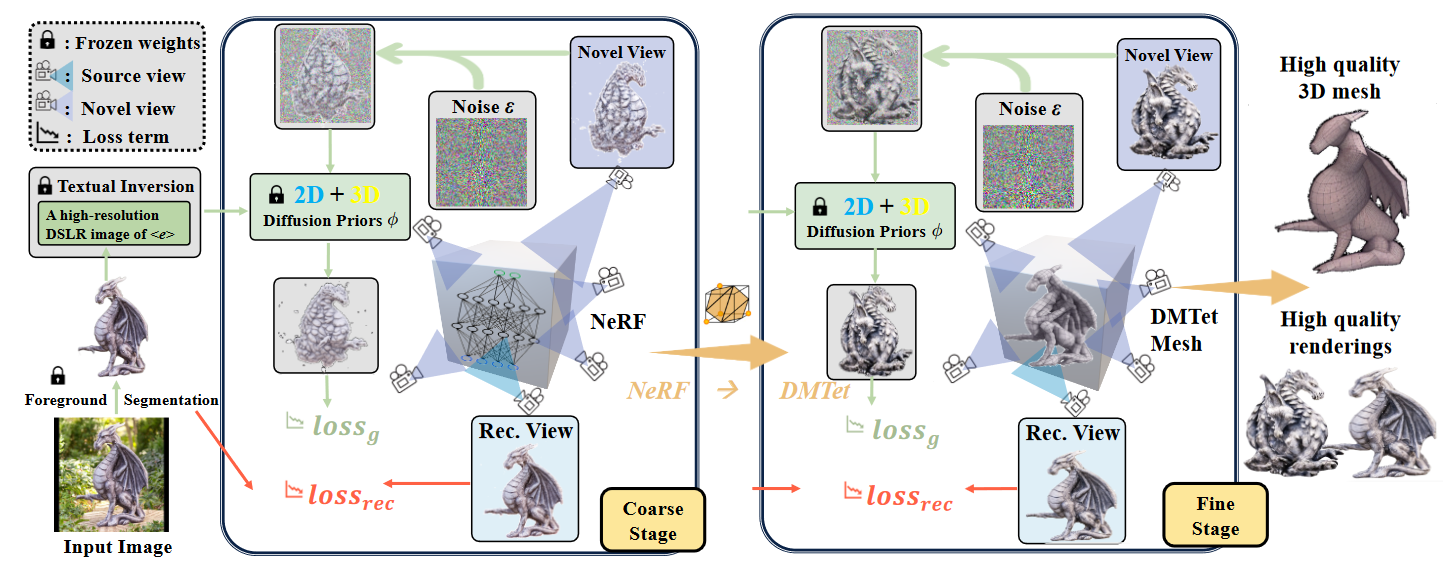
\includegraphics[width=1\columnwidth]{figures/Magic123.png}
    \caption{Overview of Magic123's two-stage process, which starts with the initial image and illustrates the transition from coarse geometry capture with Instant-NGP to high-resolution mesh refinement using DMTet. Image taken from \citep{qian2023magic123}.}\label{fig:figureMagic123}
\end{figure}


In the coarse stage, Magic123 focuses on capturing the underlying geometry that from the extracted object. It uses Instant-NGP as the Neural Radiance Field (NeRF) implementation due to its enhanced memory efficiency. The training approach in this initial phase involves a sequential process where the model first samples from the Instant NGP representation. Following this, the model undergoes optimization using multiple loss functions. The Reference View Reconstruction Loss, \(\mathbf{L}_{rec}\), ensures that the image rendered by the NeRF from a predetermined viewpoint closely aligns with the reference image from the diffusion model Stable Diffusion \citep{rombachStableDiffusion}. Alongside, the Novel View Guidance Loss, \(\mathbf{L}_{g}\), is employed. This loss function uses both 2D and 3D diffusion priors to aid in creating novel views of the object. It guides the training process towards more accurate results \citep{qian2023magic123}. Additionally, depth prior and normal smoothness are implemented to overcome inherent challenges in reconstructing 3D content from 2D images, such as avoiding flat or caved-in geometries and smoothing high-frequency artifacts on object surfaces. Despite these advanced techniques, the coarse stage faces a limitation in terms of resolution. Even with Instant-NGP, the maximum resolution achievable in the image-to-3D pipeline is capped at \(128 \times 128\) on a 16GB memory GPU \citep{qian2023magic123}.

The fine stage aims to refine the 3D model into a high-resolution mesh using Deep Marching Tetrahedra (DMTet) \citep{qian2023magic123,shen2021DMTet}. This stage effectively disentangles geometry and texture, overcoming the resolution limitations of the coarse stage and enabling the generation of meshes at a much higher resolution. The fine stage mirrors the coarse stage in structure but is distinguished by its use of DMTet for the 3D representation and loss evaluation using the viewpoint-conditioned diffusion model Zero-1-to-3 \citep{liu2023zero1to3}, where both significantly enhance the level of detail and realism in the final model \citep{qian2023magic123}.

Both stages of Magic123 use both 2D and 3D priors to guide the generation of novel views. The 2D priors, powered by Stable Diffusion, excel in imaginative extrapolation and contribute to exploring the space of possible geometries. However, they are constrained by their limited understanding of three-dimensional structures, leading to issues like unrealistic geometries or inconsistencies in textures \citep{qian2023magic123}. Contrastingly, the used 3D priors generated by viewpoint-conditioned Zero-1-to-3, provide a more accurate and consistent representation of three-dimensional objects. These priors excel in maintaining geometric fidelity but can struggle with generalizing to less common objects, sometimes resulting in oversimplified geometries.~\citep{qian2023magic123}.
